\documentclass[runningheads,a4paper]{llncs}

\usepackage{amssymb}
\setcounter{tocdepth}{3}
\usepackage{graphicx}

\usepackage{array}
\newcolumntype{P}[1]{>{\centering\arraybackslash}p{#1}}
\graphicspath{ {img/} }
\usepackage{graphicx}
\usepackage{boldline}

\usepackage{url}
\urldef{\mailsa}\path|researcher1@example.com, researcher2@example.com, researcher3@example.com|
\newcommand{\keywords}[1]{\par\addvspace\baselineskip
\noindent\keywordname\enspace\ignorespaces#1}

\begin{document}

\mainmatter  % start of an individual contribution

\title{A case study on\\
a new method of carrying a cat}

\titlerunning{A case study on something}

\author{Researcher1 (0000-0000-1111-1111)
\and Researcher2 (0000-0001-1111-2222)\and Researcher3 (0000-0001-2222-1111)}
%
\authorrunning{A case study on something}

\institute{ITMO University, Saint-Petersburg, Russia\\
\mailsa\\
\url{http://www.ifmo.ru}}

\maketitle


\begin{abstract}
  Authors describe results of their ongoing work to research a very important
  problem domain related to something. The paper presents a method and apparatus
  designed to carry a cat.
\keywords{research, data mining, big data}
\end{abstract}


\section{Introduction}

Cat carrying technology field is one of the fastest growing industries today.
Many people use cat carriers to bring their cats outside \cite{item01}.
Cat carrier products that are on the market currently do not meet demanding
requirements of the modern society.

We performed a deep research in cat carrying problem domain and developed a new
very effective technology of carrying a cat.

\section{Related works}

Traditional cat carriers are classified and described in details in
\cite{item01}, \cite{item02}. Authors of \cite{item03} discuss effectiveness of traditional methods. 

\section{Description of experiment}

A traditional method of carrying a cat is presented on Fig.~\ref{fig:TraditionalCatCarrier}.

%
\begin{figure}
	\centering
	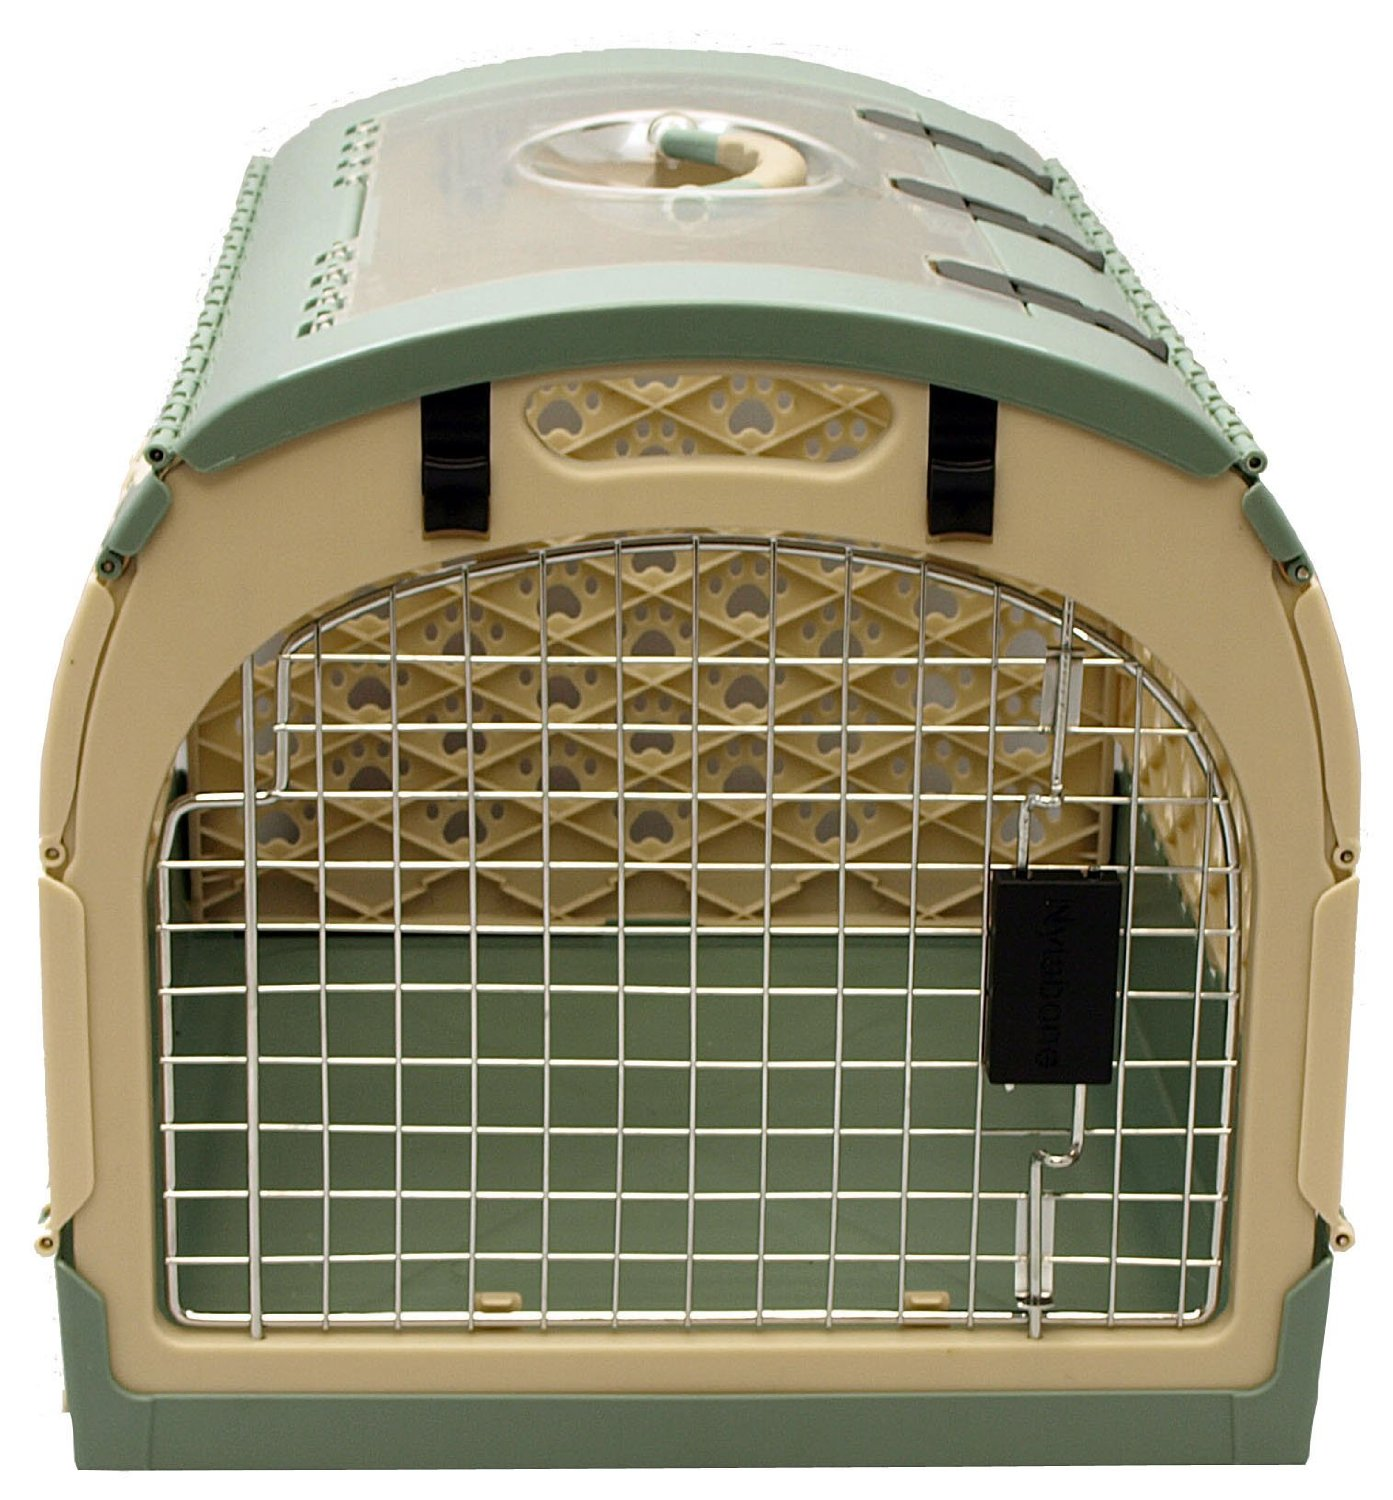
\includegraphics[width=\linewidth]{TraditionalCatCarrier}
	\caption{A traditional cat carrier}
	\label{fig:TraditionalCatCarrier}
\end{figure}
%

The traditional cat carrier is heavy and not space-efficient. While it is
possible to use modern materials to build a lighter carrier in traditional
style we decided to design a cat carrier which consists of less parts.

A proposed design is shown on Fig.~\ref{fig:NewCatCarrier}. It is much simpler
and lighter than the traditional one. It is adjustable to handle a cat of any
size, even a Maine Coon.

%
\begin{figure}
	\centering
	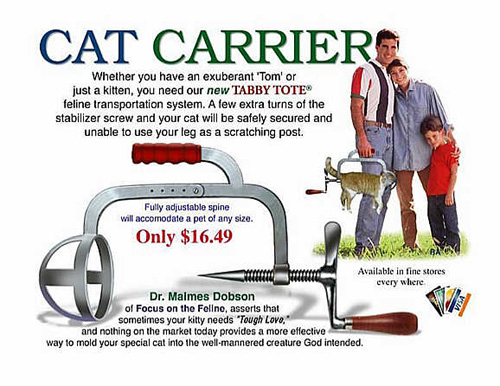
\includegraphics[width=\linewidth]{NewCatCarrier}
	\caption{A proposed cat carrier}
	\label{fig:NewCatCarrier}
\end{figure}
%

\section{Tools}

We used a male 6 years old cat in our experiment. It weighted 5.54 kilograms. We
used a traditional cat carrier produced by Cat Carriers Inc.

Authors also build their own experimental cat carrier using materials bought in
Walmart store.

\section{Results}

No cats ot other pets were harmed during our experiment. We defined a set of
metrics and conducted a survey of 20 randomly selected cat owners.

Combined comparison results are presented in Table~\ref{tab:compare}. We planned directions of future work based on these results.

%
\begin{table}
	\caption{\label{tab:compare}Comparison of traditional and new cat carriers}
	\begin{center}
		\begin{tabular}{p{5cm}|P{2.5cm}|P{2.5cm}}
			\hline
			~                              & Traditional & New \\ \hlineB{2}
			Weight                         & 3Kg     & 1Kg      \\ \hline
			Pet happiness                  & -    & +      \\ \hline
			Ability to carry two cats      & +     & -      \\ \hline
			Space effectiveness            & -   & +      \\ \hline
		\end{tabular}
	\end{center}
\end{table}
%

\section{Future work}

Authors are going to implement a fully autonomous cat carrying system utilizing
a deep learning algorithm.

We will also try to reduce the weight of our existing solution further. 

\section{Conclusion}

A problem of carrying a cat effectively and in style is actual
at the moment and will become even more actual in the future. There is a huge
demand of cat carrying systems which can work 24*7*365 in hard conditions.

Authors presented an innovative solution and performed field testing. The new
tool is better than existing methods of cat carrying by 146\%.

\begin{thebibliography}{4}

\bibitem{item01} Researcher5, R.R.: Problems of carrying a cat. J. Nature. 1 (200), (2010)

\bibitem{item02} Researcher6, R.R.: Introduction to carrying a cat. NN
  Publishing, New York (2008)

\bibitem{item03} Researcher7 R. et al.: Carrying a cat
  effectively. In: Proceedings of the Nth international
  conference on Cat Carrying, pp. 200--210. Cat Carriers Society (2011)

\bibitem{item04} Google, \url{https://google.com}

\end{thebibliography}

\end{document}
